\documentclass[conference,a4paper,twocolumn]{IEEEtran}
\usepackage{graphicx}
\graphicspath{{images/}}
\DeclareGraphicsExtensions{.png,.jpg,.pdf}
\usepackage{ifpdf}
\usepackage{cite}
\usepackage{todonotes}

\ifCLASSINFOpdf
  % \usepackage[pdftex]{graphicx}
  % declare the path(s) where your graphic files are
  % \graphicspath{{../pdf/}{../jpeg/}}
  % and their extensions so you won't have to specify these with
  % every instance of \includegraphics
  % \DeclareGraphicsExtensions{.pdf,.jpeg,.png}
\else
  % or other class option (dvipsone, dvipdf, if not using dvips). graphicx
  % will default to the driver specified in the system graphics.cfg if no
  % driver is specified.
  % \usepackage[dvips]{graphicx}
  % declare the path(s) where your graphic files are
  % \graphicspath{{../eps/}}
  % and their extensions so you won't have to specify these with
  % every instance of \includegraphics
  % \DeclareGraphicsExtensions{.eps}
\fi

\usepackage[cmex10]{amsmath}
\interdisplaylinepenalty=2500

\usepackage{algorithmic}
\usepackage{array}
\usepackage{mdwmath}
\usepackage{mdwtab}
\usepackage{eqparbox}
\usepackage[tight,footnotesize]{subfigure}
\usepackage[caption=false]{caption}
%\usepackage[font=footnotesize]{subfig}
\usepackage{fixltx2e}
\usepackage{color}
\usepackage{mathtools}


% correct bad hyphenation here
\hyphenation{op-tical net-works semi-conduc-tor}


\begin{document}
\title{DC Link Capacitor Optimization for Integrated Modular Motor Drives}
\author{\IEEEauthorblockN{Mesut Uğur}
\IEEEauthorblockA{Department of Electrical and Electronics Engineering\\
Middle East Technical University\\
Ankara, Turkey\\
Email: ugurm@metu.edu.tr}
\and
\IEEEauthorblockN{Ozan Keysan}
\IEEEauthorblockA{Department of Electrical and Electronics Engineering\\
Middle East Technical University\\
Ankara, Turkey\\
Email: keysan@metu.edu.tr}
}
\maketitle


\begin{abstract}
%\boldmath
In this paper, selection of optimum DC link capacitor for Integrated Modular Motor Drives (IMMD) is presented. First, a review of IMMD technologies is given and current research and future prospects are studied. Inverter topologies and gate drive techniques are evaluated in terms of DC link performance. The urge for volume reduction in IMMD poses a challenge for the selection of optimum DC link capacitor. DC Link capacitor types are discussed and critical aspects in selecting the DC links capacitor are listed. Analytical modeling of DC link capacitor parameters is performed and it is verified by simulations conducted using MATLAB/Simulink. Optimum selection of DC link capacitor is achieved based on the electrical, thermal and economical model.
\end{abstract}


\IEEEpeerreviewmaketitle


% \cite{Ueda2014a}
%\todo[inline]{Introduction tumuyle eksik}



\section{Introduction}


In conventional motor drive systems, drive units are placed in a cabinet and connected to the motor by means of long cables. Placing the motor and its drive separately increases the volume and weight of the system decreasing the system power density. In aerospace and electric traction applications, the motor drives are fundamental elements and power density plays an important role in the design \cite{LoCalzo2016,Wolmarans2008,Hennen2012,Lambert2015a,Lambert2015b,Galassini2015}. In addition, due to the long connection cables, high voltage transients on the motor windings caused by PWM operation occurs on the motor terminals causing leakage currents through stator winding insulation, which cause aging of insulations and shorten the motor lifetime \cite{Wang2013,Jahns2014}. One counter-measure for this effect is the utilization of filters between motor and drive, which are bulky and costly \cite{LoCalzo2016}.

In recent years, a new concept called Integrated Modular Motor Drives (IMMDs) has emerged to overcome the aforementioned problems. This concept suggests that, the drive stage of a motor drive system including the power stage, control electronics, passive elements and heatsink can be integrated into the motor resulting in a single integrated unit \cite{LoCalzo2016}, which brings several advantages. The power density of the motor drive system is significantly increased \cite{Lambert2015a,Wang2013}. A cost reduction of 20-40\% with integration is possible due to the elimination of separate enclosures and cables \cite{LoCalzo2016}. Furthermore, the long cables are eliminated so that the lifetime of the motor is increased and EMI problems are minimized \cite{Wolmarans2008}. In addition, this concept aims to modularize the overall system, dividing it into several identical parts, which share the total power equally. This technique significantly increases the fault tolerance of the motor and the drive as the system can continue its operation even if a fault occurs on one of the modules \cite{Hennen2012,Galassini2015,Wang2013}. In \cite{Wolmarans2008}, fault modes for both machine and power electronics are investigated and increase of fault tolerance for IMMDs has been shown. Moreover, the voltage stress on each module and motor winding group is reduced, which also enables the utilization of power semiconductor devices with low breakdown voltage ratings \cite{Wang2014,Wang2015}. The thermal performance of the drive is also improved as the heat sources in the system are now distributed on a larger surface area, and hot spot temperatures are reduced. In addition, fabrication, installation, maintenance and repair costs are also reduced thanks to the modular structure \cite{LoCalzo2016,Hennen2012,Lambert2015b,Jahns2014}.

Alongside of these benefits, integration of the motor and drive introduces several challenges \cite{LoCalzo2016,Wang2015}. First of all, fitting all the drive components in such a small volume requires size optimization and optimum placement of components. Moreover, cooling of motor and drive together is very difficult and detailed thermal analysis is required as presented in \cite{Lambert2015b}. In addition, the electronics is directly subjected to the physical vibration caused by the motor. In \cite{Hennen2012}, influence of machine vibration and noise to the power electronics has been investigated for a 67 kW IMMD prototype with 5-phase switched reluctance motor. To demonstrate the thermal, vibrational and EMI effects to the electronics caused by the motor, a 10 pole permanent magnet machine prototype was developed with 6 stator phases in \cite{Jahns2014}. To reduce the size of passive elements, increasing the operation frequency by the utilization of new generation wide bandgap (WBG) power semiconductors is proposed \cite{Lambert2015a,Wang2015}. Efficiency of 99.3\% has been achieved for a 900 W motor drive application with GaN power FETs \cite{Morita2011}. By increasing frequency, parasitic inductances on both power stage and gate drive circuitry become more significant, which requires careful layout design \cite{LoCalzo2016}. 

Reduction of DC link capacitor volume is very critical in IMMD design. In motor drive systems, DC link capacitors constitute a significant portion of the overall volume and the limited converter space in IMMDs makes the optimization of DC links capacitors essential. In \cite{Su2010,Bianchi2003,Zhang2010}, methods such as DC link analytical modeling, evaluation of capacitor types and their comparison, application of interleaving technique for size reduction are presented. DC link capacitor selection procedure specific to IMMDs is presented in \cite{LoCalzo2016,Wang2014,Wang2015}.

In this paper, DC link modeling is studied for an IMMD and optimum capacitor selection for the DC link is achieved based on a selection algorithm. Commercial off-the-shelf capacitor types suitable for IMMD applications have been listed and compared in terms of current ripple, cost, power density, volume and thermal performance. Effect of interleaving on capacitor RMS current ripple is analyzed.



\section{immd technology review}

\subsection{The Concept of IMMD}

There are several ways for integration of motor drive and motor proposed in the literature \cite{LoCalzo2016,Wolmarans2008}. For surface mount integrated motors, motor drive is mounted on the case of the motor, which is the most common integration type. High power integrated motor drives (IMDs) have been achieved commercially with this technique, whereas this type of integration lacks the benefits of modularity. Another technique is called end plate mount integration.

The IMMD concept mentioned in this paper has the stator iron mount type integration, which add modularity to the system. In this configuration, the system is composed of three main parts, which constitute one module of the system: a segmented stator pole piece, a concentrated coil and the power converter and its controller dedicated to that pole piece. Two examples of this IMMD configuration are shown in Fig. \ref{fig1} \cite{LoCalzo2016,Wang2015}.


\begin{figure}[h]
  \centering
  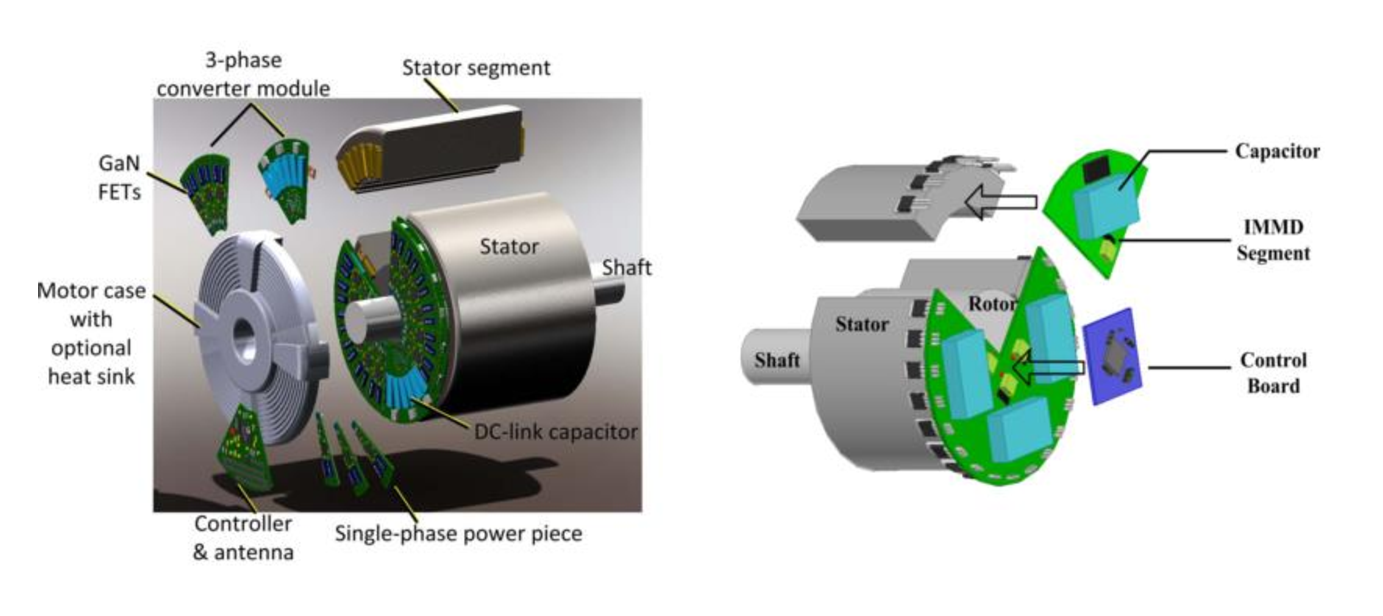
\includegraphics[width=9cm]{fig1}
  \caption{Integrated Modular Motor Drive Examples \cite{LoCalzo2016,Wang2015}}
  \label{fig1}
\end{figure}

In a conventional motor, the stator coils in different poles are usually connected in series forming a single winding for each phase. In a modular motor design, these pole windings can be connected to separate drive inverters, which are called split winding machines \cite{Galassini2015,Wang2013,Wang2015}. Split winding machine configuration brings modularity to the system and increases redundancy and fault tolerance. It also increases the flexibility of the design since various connections of separate motor drive inverter modules are possible. Complex interconnections are not required so that end winding cost and losses will also reduce \cite{Wang2015}. The segmented stator is usually formed with concentrated coils, which brings ease of manufacturing \cite{Lambert2015a}.

In IMMDs, connection of the inverters in parallel and/or series on the DC link in a variety of combinations is possible without the practical concerns related to circulating currents between inverters, since the load side is inherently isolated due to split winding machine configuration. With modular machine, the voltage level on each segment will be small supposing that the total number of turns is preserved. Presence of a high voltage on DC link will require some sort of series connection of converters or power switches in a multileveled structure. In addition, keeping the voltage level of each inverter module small will lead to the possibility of utilizing low voltage power semiconductors, which will surely enable using new generation high electron mobility transistors (HEMT) such as Gallium Nitride (GaN) \cite{Wang2015}. Furthermore, reduction of the voltage rating of each power device yields a reduction on the switching losses of the overall system \cite{LoCalzo2016}. Utilization of such low voltage devices leads to a multilevel converter in case of using a passive rectifier where the available DC link voltage is fixed \cite{Wang2013}. Many multilevel converter topologies have been proposed in the literature \cite{Wang2014}. The most common ones are Neutral Point Clamped (NPC), Flying Capacitor (FLC), Cascaded H-Bridge (CHB) and Modular Multilevel Converter (MMC). These methods have been discussed and compared in \cite{LoCalzo2016,Wang2014,Wang2015}.

The major limitation for topologies having series connection is reduced fault tolerance \cite{Galassini2015}. One of the main ideas behind modularity is to enhance the fault tolerance of the system, so it is not wise to use a fully series connected topology. On the other hand, fault tolerance on the motor drive is guaranteed for topologies with parallel connection \cite{Galassini2015}. Moreover, voltage balancing is required for series connected multilevel type converters.

It is also possible to construct a topology by just simply connecting several 3-phase 2-level modules, each of which is responsible for one stator winding module, in series and parallel according to the need for voltage and current sharing. This type of topology has the advantage of flexibility in the design, absolute symmetry, redundancy and better fault tolerance on motor drive stage. The simple structure also eliminates the need of any additional circuit components. The number of series connected modules can be determined by the relation between DC link voltage level and the breakdown voltage level of the power semiconductor devices. Once it is fixed, according to the determined pole number of the motor, number of parallel connected converters can be selected.

WBG power semiconductor devices are good candidates for IMMD applications thanks to their low on-state resistance, high switching speed and high maximum junction temperatures \cite{Morita2011}. For traditional silicon devices such as Insulated Gate Bipolar Transistor (IGBT), switching frequency is usually limited to 20 kHz \cite{Lambert2015a}. With Silicon Carbide (SiC) MOSFET and GaN, switching frequencies up to 100 kHz can be used in applications with tens of kWs [10, 13] \cite{Wang2015,Morita2011}. In IMMD prototype examples, GaN transistors have been widely utilized due to their very low on-state resistance, which reduces conduction loss drastically, very high switching speed, which enables size reduction for passive elements, and good thermal performance. Moreover, GaN devices do not need external free-wheeling diodes as their reverse conduction performance is good. Their efficiency in IMMD applications has been proven to be good, not only at rated power, but also in the whole output power range \cite{Morita2011}. In \cite{Wang2015}, GaN transistors with 200 V breakdown voltage rating were utilized at 40 kHz switching frequency in an IMMD prototype where no heatsink was required. On the other hand, due to low voltage rating of a single device, series connected multilevel converter topology had to be utilized \cite{Wang2013}.

\subsection{DC Link capacitor studies}

DC link characterisation and capacitor selection for three-phase motor drive applications has been studied several times. In \cite{Bianchi2003} and \cite{Lee2007}, duties of DC link capacitors are listed in a conventional motor drive inverters. DC link capacitors mainly supplies the fluctuating power frequency of which is six times the grid frequency in case of passive diode bridge rectifiers are used, supplies the inverter current at switching frequency, supplies the transient power deviations and supplies the necessary hold-up energy in case of power shutdown \cite{Bianchi2003}.

In \cite{Lee2007}, analytical modeling of DC link considering both input rectifier and motor drive inverter has been presented for asjustable speed drive (ASD) applications. DC link capacitor stress under unbalanced grid voltages and grid voltage sag conditions has also been studied. Aluminium electrolytic capacitors has been considered and their failure modes has been investigated. DC link average current and RMS current expressions have been formulated to analyze the capacitor requirement \cite{Bianchi2003} \cite{Gohil2014} \cite{Rixin2007}. In \cite{Rixin}, capacitance requirement is given analytically in case of voltage dips in the grid for a general back-to-back converter consisting of active three-phase PWM converters at both sides.

Aluminium electrolytic capacitor is the most commonly used type of capacitors in motor drive applications due to its low cost, large capacitance per volume and ride-through energy storage capability \cite{Lee2007}. On the other hand, reliability, limited lifetime and dependency on the operating conditions are major concerns. Therefore, among several parameters for the selection of aluminium electrolytic capacitors for DC link applications, capacitor size is usually determined by its life span \cite{Lee2007}. A thermal model has been proposed and the effect of operating temperature, operating voltage and current on the capacitor lifetime and failure rate has been studied in \cite{Bianchi2003} \cite{Gohil2014}. 


DC link ripple characterisation has been achieved for conventional motor drive systems in terms of pulse width modulation (PWM) methods in \cite{Gohil2014} and effect of interleaving and phase shifting is investigated. Reduction of DC link capacitor stress with shifted control and PWM carrier signal phase-shifting is analyzed in detail for a double three-phase motor drive unit \cite{Basler2015}. The DC link capacitor current at different modulation index values and PWM phase-shift angles is analyzed. Optimum phase-shift angle is investigated for minimum capacitor RMS current.

DC link capacitor selection for IMMD applications has also been studied in a few papers. In \cite{Engelmann2015}, a 30kVA integrated motor drive has been proposed and implemented. A six-phase H-bridge motor drive topology has been proposed where power stage printed circuit boards (PCB) are placed inside the motor housing. A modular structure is utilized to decrease the DC link capacitor voltage requirement. A capacitor bank composed of hundreds of SMD ceramic capacitors is used for each module to overcome size constraints. Application of interleaving with a modular multilevel inverter topology for an IMMD application has been studied in \cite{Wang2014} and \cite{Wang2013} for the reduction of DC link capacitor size to enhance the power density. The aspects regarding volume reduction in the power electronics in terms of DC link capacitor bank has been discussed. Capacitor height reduction has also been emphasized \cite{Wang2013}.

Although DC link characterisation and capacitor selection topics are widely presented in the literature for motor drive inverters, very few of those studies are based on IMMD applications where major considerations are different. Volume reduction, height minimization and thermal characteristics should be taken priority. Moreover, those which consider IMMD lack a consistent modeling with several aspects. Analytical models are tam değil.

In this paper, DC link capacitor optimization is achieved for an IMMD application. Major limitations due to being integrated are considered. On the other hand, benefits due to modularization are utilized.


\cite{Engelmann2015}


\cite{Basler2015}





\section{DC LINK MODELING}


Reduction of DC link capacitor volume is very critical in IMMD design. As seen in Fig. \ref{fig2} , in a modern power electronics system, passive elements take a significant portion of overall volume and cost \cite{LoCalzo2016}. It was also stated in [12] that, in motor drive inverters, DC link capacitors constitute 20\% of cost and weigh, and 30\% of volume. The limited converter space in IMMDs makes the optimization of DC links capacitors essential. For this purpose, accurate modeling of DC link is required. Decreasing the volume of capacitors is not sufficient alone, the height of the capacitors should also be minimized as they are the tallest components in IMMDs \cite{Wang2013,Wang2015}.

\begin{figure}[h]
  \centering
  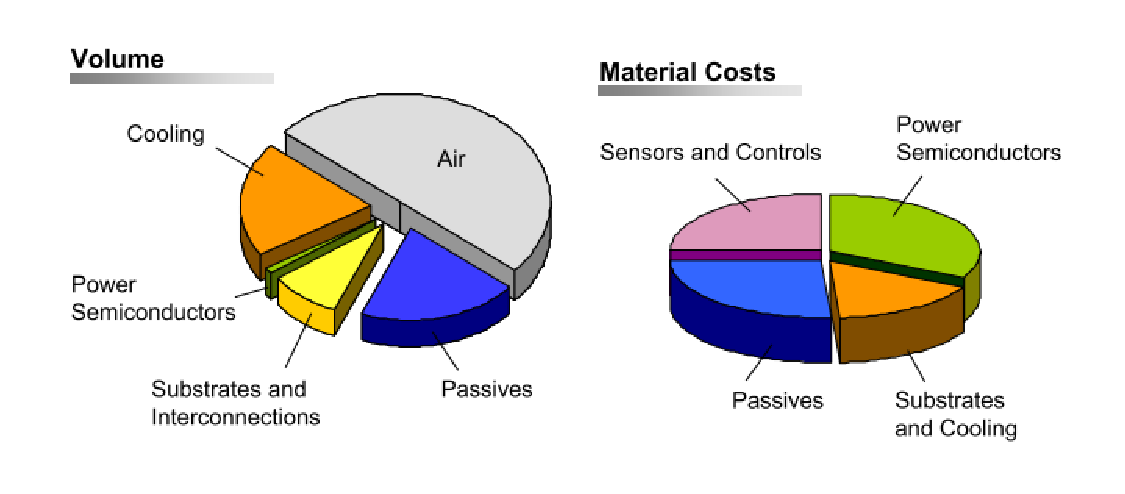
\includegraphics[width=9cm]{fig2}
  \caption{Volume and cost sharing of different parts in a modern power electronics system [1]}
  \label{fig2}
\end{figure}


\subsection{Analytical Modeling}


The fundamental parameters affecting the size of a DC link capacitor are DC voltage requirement, capacitance requirement due to DC link voltage ripple and RMS current rating requirement due to DC link capacitor current ripple. Temperature characteristics is also important as it affects the reliability and lifetime of a capacitor. 

DC link voltage, which is a parameter directly related to capacitor height, highly depends on the selected inverter topology. For multilevel converters where several converter are connected in series, DC voltage rating of each capacitor can be reduced. Actually, same thing can be done for a topology with a single DC link by just simply connected capacitors with lower voltage ratings in series. In Section 4, effect of series connection of several DC link capacitors with lower DC voltage rating is discussed. RMS current rating is directly related to the power requirement and is not effected much by the switching frequency \cite{Wang2013,Wang2015,Su2010}. Therefore, for a given converter with a specific power output, this parameter is fixed. Capacitance requirement, on the other hand, is directly related with the switching frequency. In this section, each parameter will be analytically modeled to be used in the capacitor selection algorithm. The model of the DC link to be used in this paper is shown in Fig. \ref{fig3}.
Rectifier side is considered to be an ideal DC source, denoted as $I_{in}$. The inverter DC current ($i_{dc}$) is the sum of the average current ($I_{in}$). and the ripple current which flows through the capacitor ($i_c$). The average DC current can be expressed as in \ref{eq1}, where $I_{a,peak}$ is the peak value of any line current, $m_a$ is modulation index, and φ is power factor angle.

\begin{figure}[h]
  \centering
  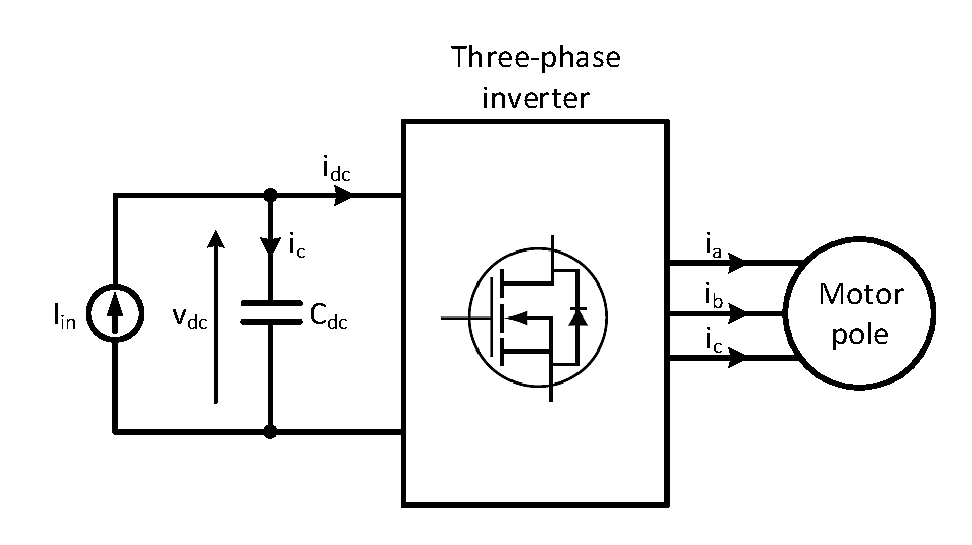
\includegraphics[width=9cm]{fig3}
  \caption{Model of the DC Link}
  \label{fig3}
\end{figure}


\begin{equation}
\label{eq1}
I_{avg} = \frac{3}{4}I_{a,peak}m_acos(\phi)
\end{equation}


The capacitor current is composed of sideband harmonics around the switching frequency and its integer multiples. The RMS value of this current has been derived in \cite{Su2010,Bianchi2003} as in \ref{eq2}, where $I_{a,rms}$ is the RMS value of any line current.

\begin{equation}
\label{eq2}
I_{c,rms} = I_{a,rms}\sqrt{\bigg[2m_a\Big(\frac{\sqrt{3}}{4\pi}+\cos(\phi)^2\big(\frac{\sqrt{3}}{\pi}-\frac{9}{16}m_a\big)\Big)\bigg]}
\end{equation}


The voltage ripple on the DC link has not been explicitly derived in the literature. Here, a method is developed to model the peak-to-peak ripple voltage by using the relation between the capacitor voltage and current, and the shape of the capacitor ripple current as shown in \ref{eq3}.


\begin{equation}
\label{eq3}
v_{dc,r,pp} = \frac{0.7(I_{a,peak}-I_{dc})m_a}{C_{dc}f_{sw}}
\end{equation}


Finally, temperature characteristics and the power loss of capacitors are modeled. The core temperature ($T_c$) of a capacitor can be expressed as in \ref{eq4}, where $T_a$ is the ambient temperature, $R_{th,c}$ is the thermal resistance of the capacitor, and $R_c$ is the ESR of the capacitor, which is a parameter dependent on the core temperature of the capacitor as shown in \ref{eq5} \cite{Bianchi2003}. As seen from these equations, ESR of the capacitor $R_c$ is a temperature dependent parameter so that the thermal model is an implicit equation and should be treated so.


\begin{equation}
\label{eq4}
T_{c} = T_{a}+p_{c}(T_{c})R_{th,c}
\end{equation}


\begin{equation}
\label{eq5}
p_{c} = I_{c,rms}^2R_{c}(T_c)
\end{equation}


\subsection{Effect of Interleaving}

Interleaving is widely used in power converters to decrease ripple currents and ripple voltages for passive component size reduction \cite{Zhang2010}. IMMD system is suitable for the application of interleaving as there are multiple converter modules, which can be connected in different configurations. It is a well-known fact that, phase shifting applied to the converters which are interleaved reduces the capacitor current ripple and DC link voltage ripple \cite{LoCalzo2016,Wang2015,Su2010}. In \cite{Wang2015}, interleaving has been applied to an IMMD prototype switching frequency of which is 100 kHz. The effect of interleaving to the DC link current waveform and the RMS value of the capacitor current in motor drive inverters is obtained by simulation as shown in Fig \ref{fig4}.
The rule of thumb phase shift angle to be applied to the converters is usually given as 360/n \cite{LoCalzo2016}. The percent RMS current is obtained with changing number of parallel connected modules to shown the optimum phase shift angle for each case as in Fig. \ref{fig5}. It has been shown that, minimum percent RMS current is obtained around 360/n angle for each case. It is also shown that, RMS current does not decrease significantly after a certain number of parallel connected modules, and a total number of 4 or 6 modules can be suggested.


\begin{figure}[h]
  \centering
  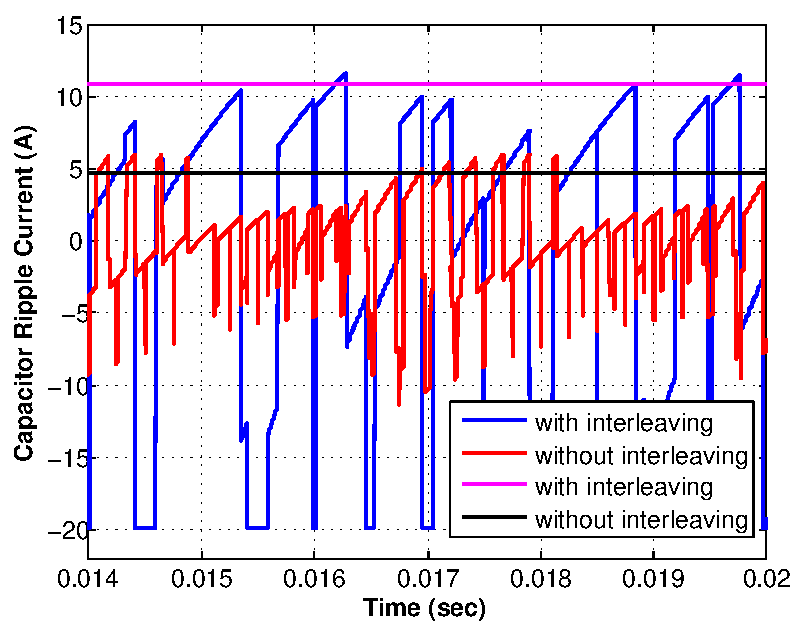
\includegraphics[width=9cm]{fig4_2}
  \caption{Effect of interleaving to motor drive inverters}
  \label{fig4}
\end{figure}


\begin{figure}[h]
  \centering
  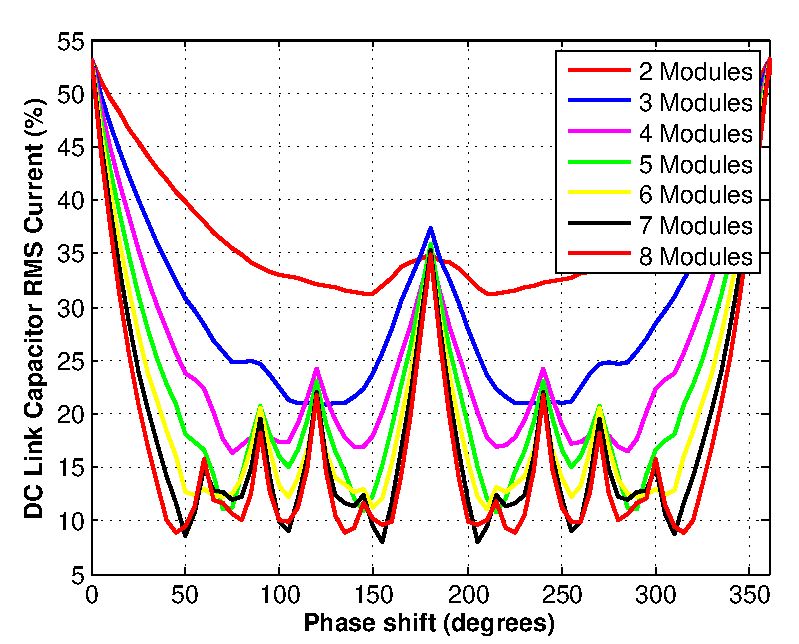
\includegraphics[width=9cm]{fig5_2}
  \caption{Capacitor percent RMS current characteristics}
  \label{fig5}
\end{figure}



\section{DC LINK CAPACITOR EVALUATION}

\subsection{Types of Capacitors}


Common capacitor types used in motor drive DC links are aluminum electrolytic capacitors, metal film capacitors and multilayer ceramic capacitors (MLCC). Comparison of these capacitors in terms of several aspects are shown in Table \ref{table1} \cite{LoCalzo2016,Lambert2015a,Wang2013,Wang2015,Brown2007}.

Aluminum electrolytic capacitors are usually preferred due to their high capacitance and low cost. On the other hand, since their RMS current ratings are low, parallel connection of multiple capacitors may be required. Reliability of these capacitors is a major concern as their lifetime and failure rate highly depend on operating temperature, voltage and current magnitudes \cite{Su2010}. When an aluminum electrolytic capacitor is operated at 90\% of its rated voltage, the failure rate reduces to 60\% \cite{Bianchi2003}. Temperature limitation is another major concern of electrolytic capacitors, which makes them unsuitable for IMMD applications \cite{Brown2007}.

Film capacitors, on the contrary, have low capacitance but high RMS current rating. Therefore, parallel connection of multiple film capacitors is required to meet the capacitance requirement. As the capacitance value can be optimized with switching frequency, which is not the case for RMS current, they are more preferable in IMMD applications. They are very reliable and durable capacitors, however they are more expensive than electrolytic capacitors.

MMLCs are low cost and high current rating capacitors, however they are not commercially available with the power rating of a DC link capacitor. Therefore, series and parallel connection of several capacitors is needed. The main problem for MLLC in IMMD applications is their sensitivity to mechanical effects such as vibration \cite{Brown2007} due to being in close proximity to the motor.



\begin{table}[h]
\renewcommand{\arraystretch}{1.4}
\caption{COMPARISON OF CAPACITOR TYPES}
\label{table1}
\centering
\begin{tabular}{|c|c|c|c|}
\hline
Property & 10 kW & Switching frequency & 20 kHz\\
\hline
Motor fund. frequency & 50 Hz & Supply frequency & 50 Hz\\
\hline
Supply voltage & 400 V & Motor voltage & 400 V\\
\hline
Three-phase modules & 4 & Parallel connected modules & 4\\
\hline
DC Bus filter inductance & 1 mH & DC bus filter capacitance & 100 uF\\
\hline
Some motor parameters & abc & Some other parameters & xyz\\
\hline
\end{tabular}
\end{table}


\begin{tabular}{ |p{4cm}||p{1cm}|p{1cm}|p{1cm}|  }
 \hline
 \multicolumn{2}{|c|}{Country List} \\
 \hline
 
 Country Name    & ISO  &ISO &ISO \\
 \hline
 Afghanistan   & AF    &AFG&   004\\
 Aland Islands&   AX  & ALA   &248\\

 \hline
\end{tabular}


\subsection{Capacitor Selection Aspects}

In motor drives, DC link capacitors have the functions of taking on the power fluctuation on the DC link occurring at two or six times the supply frequency (depending on the number of phases), supplying the current ripples at the inverter switching frequency, to avoid the injection of high frequency ripples from one side to the other in the back-to-back structure (decoupling), to provide the drive system for a while in case of power shutdown, to supply the transient powers etc. \cite{Bianchi2003}. In this research work, rectifier side is considered as an ideal DC current source so that the only frequency components observed on the DC link will be composed only inverter side harmonics. Normally, superposition should be used considering both the harmonic contributions of both inverter side and rectifier side \cite{Bianchi2003}.
The basic parameters affecting the selection of DC link capacitor are:

\begin{itemize}
  \item Capacitance requirement due to DC link voltage ripple
  \item RMS current rating requirement due to DC link capacitor current ripple
  \item Voltage rating due to DC link voltage and topology
\end{itemize}

In addition, for an IMMD system, the major concerns for the DC link capacitor selection can be listed as follows:

\begin{itemize}
  \item High power density due to size constraints
  \item Low height
  \item Low cost
  \item Low temperature sensitivity
  \item Mechanical durability due to being in close proximity to the motor
  \item Low reduction in lifetime due to operating conditions
\end{itemize}


\subsection{Capacitor Selection Algorithm}

Based on the analytical models developed so far, capacitor datasheets, capacitor selection aspects and simulation work, an algorithm for the optimization of DC link capacitor for an IMMD application is developed and implemented. The basic flowchart of the algorithm can be seen in Fig. \ref{fig6}. The algorithm takes the inputs which define the operating conditions and ratings of the motor drive, takes the limitations as constraints and use them in the calculation of critical variables. The capacitor RMS current requirement is calculated with modulation index being variable to cover the whole operating region. Switching frequency is also considered as a variable parameter to give the designer flexibility, which is then used in capacitance requirement calculation. Datasheet parameters are fed to the algorithm to check the performance of different capacitors with the given constraints. The number of capacitors to be connected in parallel is determined for each type. In addition to this procedure, capacitors with different voltage ratings are also considered to observe the effect of using multiple series connected capacitors.



\begin{figure}[h]
  \centering
  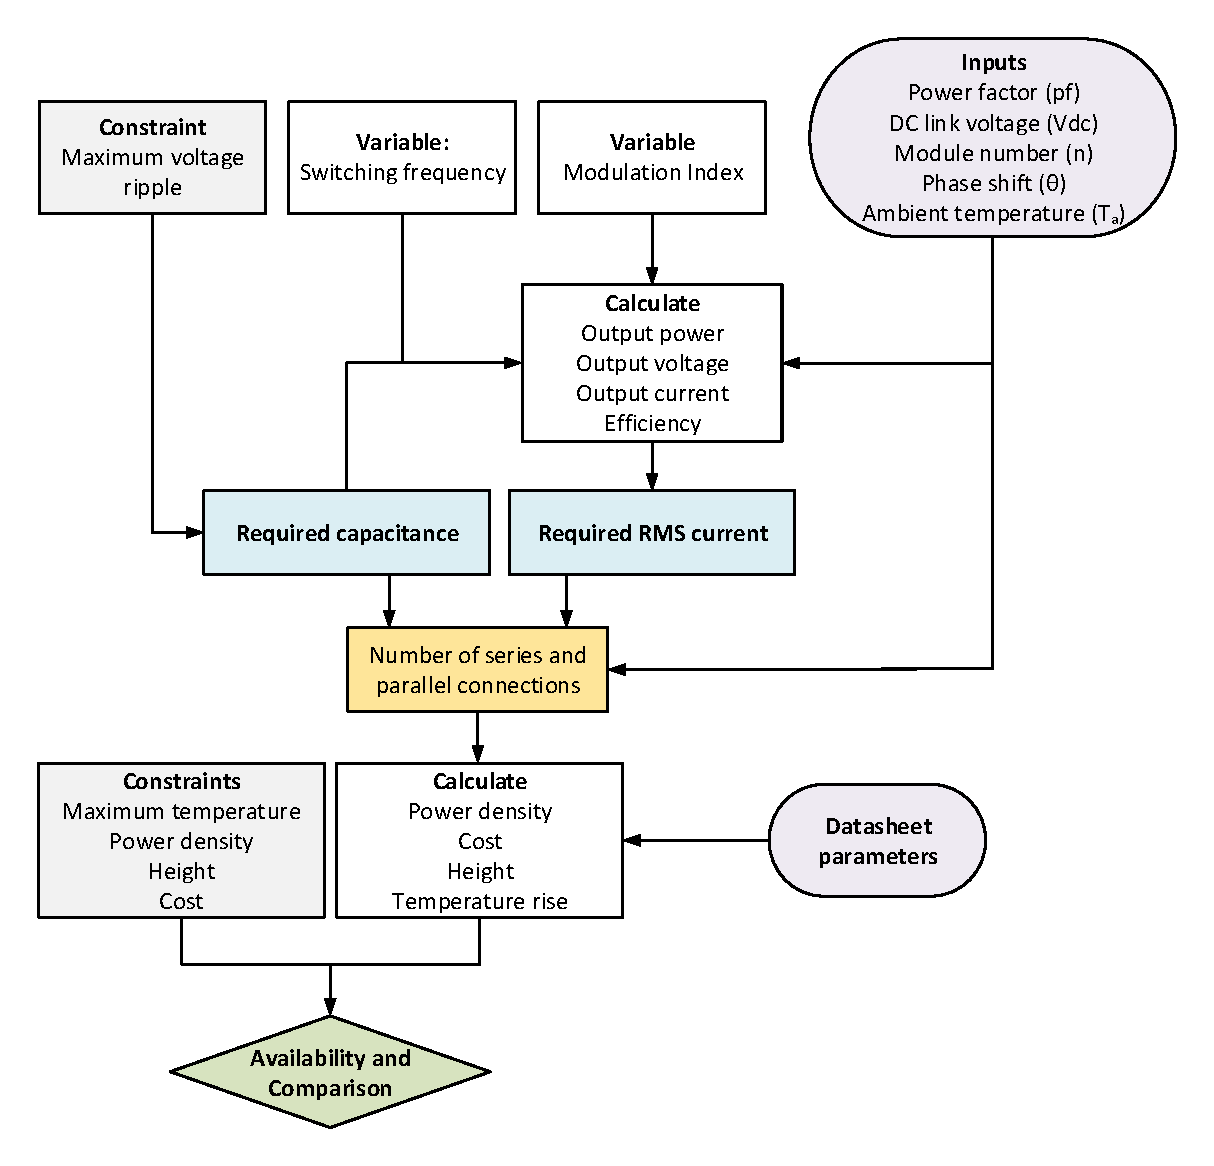
\includegraphics[width=9cm]{fig6}
  \caption{Flowchart of the optimum capacitor selection algorithm}
  \label{fig6}
\end{figure}



\section{Results}

The results obtained by using the algorithm and a set of film capacitors from [16] and presented in this section. The system parameters and constraints used in the algorithm are listed in Table \ref{table2}. In Fig. \ref{fig7}, RMS current requirement for different modulation index values are obtained. In Fig. \ref{fig8}, capacitance requirement for different switching frequencies are obtained considering the modulation index at the worst condition. It has been shown that increasing the switching frequency above 100 kHz does not have much effect on the capacitance requirement. Moreover, after this point, the RMS current requirement becomes more dominant for film capacitors. Moreover, the maximum RMS current requirement occurs around 0.8 modulation index, which has been taken as the actual requirement. Effect of frequency to the RMS current is negligibly small, and it is not included in the analysis and results.



\begin{table}[h]
\renewcommand{\arraystretch}{1.4}
\caption{System parameters and constraints}
\label{table2}
\centering
\begin{tabular}{|c|c|c|c|}
\hline
Total output power & 10 kW & Switching frequency & 20 kHz\\
\hline
Motor fund. frequency & 50 Hz & Supply frequency & 50 Hz\\
\hline
Supply voltage & 400 V & Motor voltage & 400 V\\
\hline
Three-phase modules & 4 & Parallel connected modules & 4\\
\hline
DC Bus filter inductance & 1 mH & DC bus filter capacitance & 100 uF\\
\hline
Some motor parameters & abc & Some other parameters & xyz\\
\hline
\end{tabular}
\end{table}


\begin{figure}[h]
  \centering
  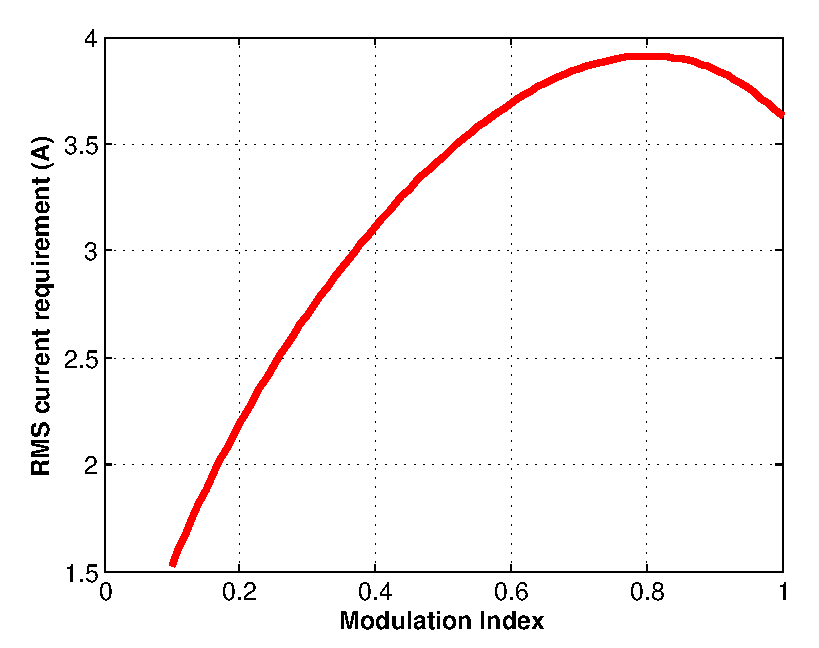
\includegraphics[width=9cm]{fig7_2}
  \caption{RMS current requirement vs modulation index}
  \label{fig7}
\end{figure}


\begin{figure}[h]
  \centering
  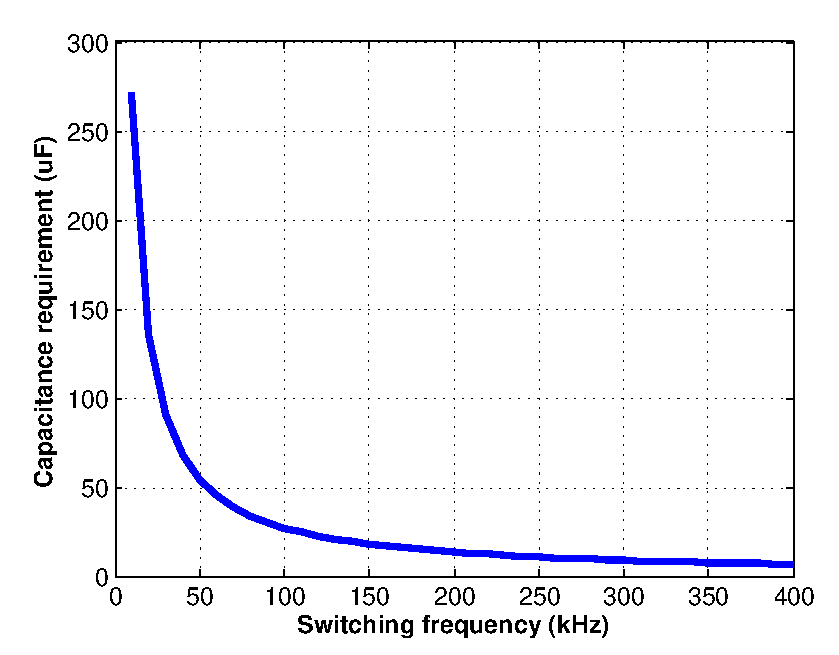
\includegraphics[width=9cm]{fig8_2}
  \caption{Capacitance requirement vs switching frequency}
  \label{fig8}
\end{figure}

Two sets of capacitors, having 25 different capacitors each, were selected from the same datasheet [16], which have voltage rating of 300V and 450V. The algorithm was implemented on these sets and number of series and parallel connections needed for each type of capacitor is found. Some samples from the capacitors are selected and listed in \ref{table3}, and compared, which was achieved with 40 kHz switching frequency. The suitable capacitors according to the selected constraints are highlighted on Table \ref{table3}.

Using a single capacitor with large capacitance and large voltage rating (Cap no.12) seems to be a good choice at the first glance as it has a very good power density, low height and lowest cost; however, it has the highest temperature rise since its surface area is too small. On the other hand, using high number of capacitors having low capacitance and low voltage rating (Cap no.1, 2, and 3) gives best thermal performance and lowest height, but their power density is too small and cost increases with this configuration. It can also be deduced that using high number of series connections and low number of parallel connections (Cap no. 4, 5) yields the worst results in terms of all the constraints.

For 450V capacitors, selecting capacitors with low capacitance (Cap no. 6, 7) is not also the best choice as the cost increases due to multiple parallel connection. The best results have been obtained by capacitor no.9 which has 20 µF capacitance and 450 V voltage rating and needs 4 parallel connection.


\begin{table}[h]
\renewcommand{\arraystretch}{1.4}
\caption{Comparison of Selected Capacitors,(s: series, p: parallel)}
\label{table3}
\centering
\begin{tabular}{|c|c|c|c|}
\hline
Total output power & 10 kW & Switching frequency & 20 kHz\\
\hline
Motor fund. frequency & 50 Hz & Supply frequency & 50 Hz\\
\hline
Supply voltage & 400 V & Motor voltage & 400 V\\
\hline
Three-phase modules & 4 & Parallel connected modules & 4\\
\hline
DC Bus filter inductance & 1 mH & DC bus filter capacitance & 100 uF\\
\hline
Some motor parameters & abc & Some other parameters & xyz\\
\hline
\end{tabular}
\end{table}


\section{Conclusion}

IMMD applications is presented. Integration of the motor drive power electronics into the motor introduces several challenges for the DC link capacitor selection. On the other hand, modular structure of IMMD brings flexibility for the design and capacitor selection. Interleaving technique can be applied to reduce the DC link voltage and current ripple. Among several capacitor types, film capacitor is more suitable for IMMD DC links due to its good current ripple ratings, reliability, good thermal performance and suitability for vibrational environments. Accurate models have been developed considering electrical, thermal and economical aspects. These models are used in an algorithm to determine the best choice among a set of selected commercial film capacitors. The alternative configurations include series connection of multiple low voltage capacitors to meet the DC link voltage requirement and parallel connection of multiple low capacitance capacitors to meet the voltage and current ripple requirements.

Considering the parameters such as power density, cost, height and temperature rise, it has been shown that, using 4 20 µF, 450 V capacitors in parallel gives the best performance in all aspects for this specific application.


\bibliography{isieref}
\bibliographystyle{IEEEtran}


\end{document}